\documentclass[a4paper]{article}
\usepackage{tikz}
\usetikzlibrary{automata, positioning, arrows}
\usepackage[document]{ragged2e}

\tikzset{
->, % makes the edges directed
>=stealth', % makes the arrow heads bold
node distance=3cm, % specifies the minimum distance between two nodes. Change if necessary.
every state/.style={thick, fill=gray!10}, % sets the properties for each 'state' node
initial text=$ $, % sets the text that appears on the start arrow
}

\begin{document}


\section{Heading on Level 1 (section)}
This is an example of how to use the tikz libraries in LaTeX to draw state machine diagrams, DFAs, NFAs and Turing Machines.
\bigskip

\begin{figure}[ht] % 'ht' tells LaTeX to place the figure 'here' or at the top of the page
\centering % centers the figure


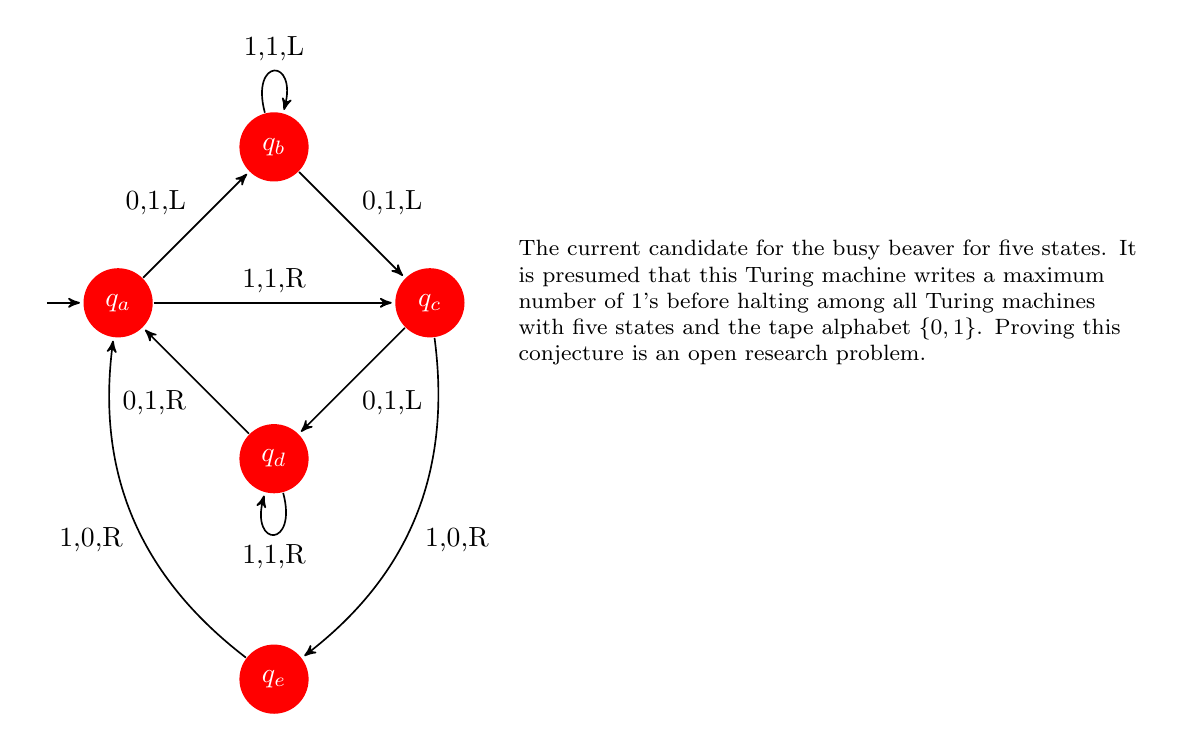
\begin{tikzpicture}[->,>=stealth',shorten >=1pt,auto,node distance=2.8cm,semithick]
\tikzstyle{every state}=[fill=red,draw=none,text=white]
\node[initial,state] (A) {$q_a$};
\node[state] (B) [above right of=A] {$q_b$};
\node[state] (D) [below right of=A] {$q_d$};
\node[state] (C) [below right of=B] {$q_c$};
\node[state] (E) [below of=D] {$q_e$};
\path (A) edge node {0,1,L} (B)
edge node {1,1,R} (C)
(B) edge [loop above] node {1,1,L} (B)
edge node {0,1,L} (C)
(C) edge node {0,1,L} (D)
edge [bend left] node {1,0,R} (E)
(D) edge [loop below] node {1,1,R} (D)
edge node {0,1,R} (A)
(E) edge [bend left] node {1,0,R} (A);
\node [right=1cm,text width=8cm,font=\footnotesize] at (C)
{
The current candidate for the busy beaver for five states. It is
presumed that this Turing machine writes a maximum number of
$1$'s before halting among all Turing machines with five states
and the tape alphabet $\{0, 1\}$. Proving this conjecture is an
open research problem.
};
\end{tikzpicture}


\caption{TM Transition Digram Example}
\label{fig:my_label0}
\end{figure}

\bigskip


\begin{figure}[ht] % 'ht' tells LaTeX to place the figure 'here' or at the top of the page
\centering % centers the figure


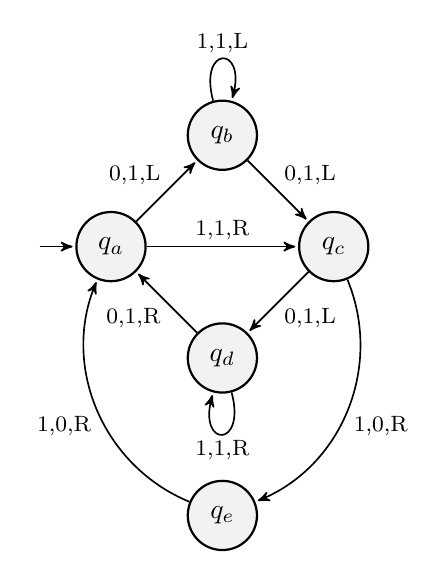
\begin{tikzpicture}[->,>=stealth',shorten >=1pt,%
auto,node distance=2cm,semithick,
inner sep=2pt,bend angle=45]
\node[initial,state] (A) {$q_a$};
\node[state] (B) [above right of=A] {$q_b$};
\node[state] (D) [below right of=A] {$q_d$};
\node[state] (C) [below right of=B] {$q_c$};
\node[state] (E) [below of=D] {$q_e$};
\tikzstyle{every node}=[font=\footnotesize]
\path (A) edge node {0,1,L} (B)
edge node {1,1,R} (C)
(B) edge [loop above] node {1,1,L} (B)
edge node {0,1,L} (C)
(C) edge node {0,1,L} (D)
edge [bend left] node {1,0,R} (E)
(D) edge [loop below] node {1,1,R} (D)
edge node {0,1,R} (A)
(E) edge [bend left] node {1,0,R} (A);
\end{tikzpicture}

\caption{Caption of the FSM}
\label{fig:my_label1}
\end{figure}


\bigskip


\bigskip

\begin{figure}[ht] % 'ht' tells LaTeX to place the figure 'here' or at the top of the page
\centering % centers the figure

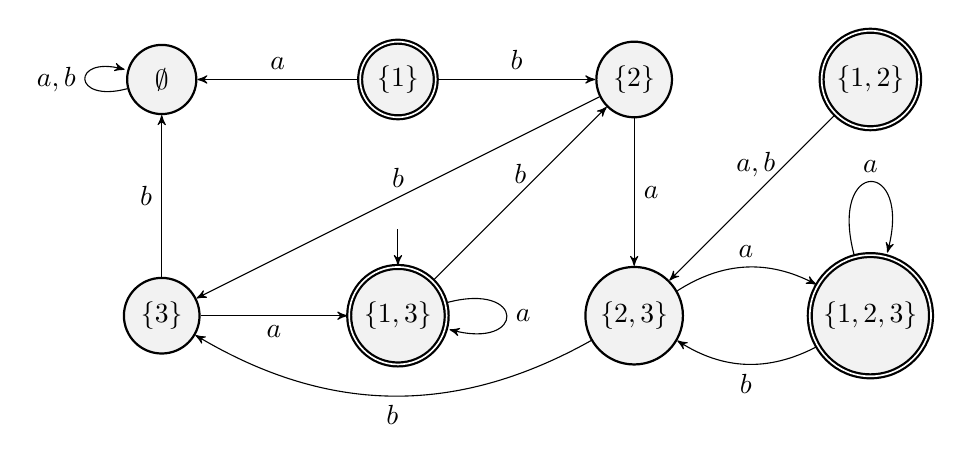
\begin{tikzpicture}
\node[state] (phi) {$\emptyset$};
\node[state, accepting, right of=phi] (1) {$\{1\}$};
\node[state, right of=1] (2) {$\{2\}$};
\node[state, accepting, right of=2] (12) {$\{1, 2\}$};
\node[state, below of=phi] (3) {$\{3\}$};
\node[state, initial, initial where=above, accepting, right of=3] (13) {$\{1, 3\}$};
\node[state, right of=13] (23) {$\{2, 3\}$};
\node[state, accepting, right of=23] (123) {$\{1, 2, 3\}$};
\draw (phi) edge[loop left] node{$a, b$} (phi)
(1) edge[above] node{$a$} (phi)
(1) edge[above] node{$b$} (2)
(2) edge[right] node{$a$} (23)
(2) edge[above] node{$b$} (3)
(12) edge[above, pos=.3, left=2pt] node{$a, b$} (23)
(3) edge[left] node{$b$} (phi)
(3) edge[below] node{$a$} (13)
(13) edge[loop right] node{$a$} (13)
(13) edge[above] node{$b$} (2)
(23) edge[bend left, above] node{$a$} (123)
(23) edge[bend left, below] node{$b$} (3)
(123) edge[loop above] node{$a$} (123)
(123) edge[bend left, below] node{$b$} (23);
\end{tikzpicture}

\caption{Caption of the FSM3}
\label{fig:my_label3}
\end{figure}



\end{document}
